\begin{figure}
    \centering
    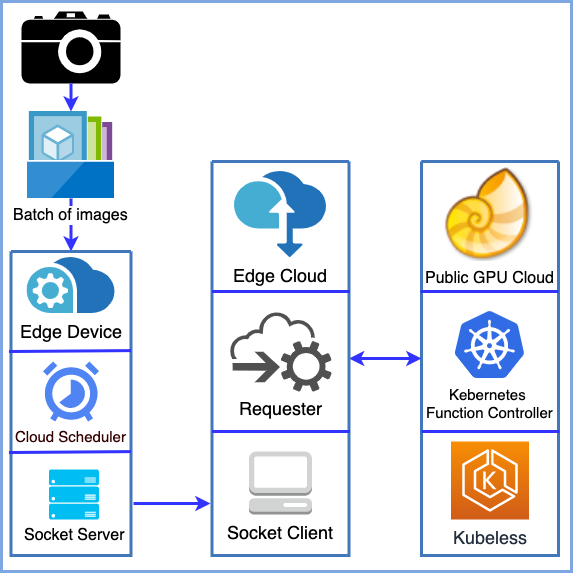
\includegraphics[scale=0.4]{STOIC}
    \caption{\textbf{The Architecture of STOIC}}
    \label{fig:STOIC}
\end{figure}

To leverage accelerator and distributed scheduling using the serverless architecture, we have developed STOIC, a framework for executing machine learning applications in hybrid cloud consisting of edge devices and public data centers. The STOIC streamlines the end-to-end process of packaging, transferring, scheduling, executing and retrieving result for machine learning applications. Figure~\ref{fig:STOIC} shows the architecture of STOIC, which is composed by three principal pillars: Edge Controller, Edge Cloud and Public GPU cloud.

\subsection{Edge Controller}
 We deploy a collection of edge devices, including multiple motion-detecting camera traps in open field and a local server as edge controller in the research facility at Sedgwick Natural Reserve~\cite{ref:sedgwick}. Across the field, especially at the water pond, we install camera traps to capture images of wildlife and they are connected by microwave link networks to edge controller in the research facility. When a motion is detected, the camera traps take photos and persist the images to the attached disk volume. Periodically, they transfer the photos to edge controller in the facility, where STOIC socket server constantly listens for batch of images and cloud scheduler assigns the task to different cloud components. 
 
 \subsection{Edge Cloud}
 
 As a intermediate layer between edge controller and public cloud, edge cloud can be placed anywhere, preferably near edge devices, to lower the latency. Currently, we built it up in our lab by a cluster of nine Intel NUCs~\cite{ref:nucs} with a direct connection over microwave radio to the edge devices at Sedgwick Natural Reserve. It is managed by Eucalyptus cloud system~\cite{ref:euca} that supports Linux virtual machine instance of Ubuntu and CentOS. Running on an instance, the STOIC socket client listens for the request from edge controller and, then, either executes the job locally on edge cloud or has STOIC requester interact with public cloud to complete the designated task.
 
 \subsection{Public Cloud}
 
 The public cloud is built on the top of Nautilus Cloud~\cite{ref:nautilus}, which is a HyperCluster research platform led by researchers at UC San Diego, National Science Foundation, Department of Energy and various participating universities globally. Being designed for running data and computation intensive applications, Nautilus uses Kubernetes~\cite{ref:k8s} as interface to manage and scale containerized applications and uses Rook~\cite{ref:rook} to automate Ceph~\cite{ref:ceph} data services. As of Nov. 2019, 141 computing nodes across the US joined Nautilus Cloud and 422 GPUs are available in the cluster. All these node are connected via a multi-campus network. We consider Nautilus as an ideal public cloud to leverage accelerator (GPUs) in serverless architecture to serve edge devices. 
 
 \subsection{Implementation}
 
 \subsubsection{Language}
 Considering performance and interface, STOIC is primarily developed in Golang, since the language provides better performance than scripting language like Python, as well as user-friendly interface~\cite{ref:client-go} to Kubernetes. 
 
 \BlankLine
 \subsubsection{Serverless framework}
 To enable Serverless architecture, STOIC employs kubeless~\cite{ref:kubeless} and Docker~\cite{ref:docker} at Nautilus Cloud. As a kubernetes-native serverless framewrok, kubeless uses CRD (Custom Resource Definition)\cite{ref:crd} to dynamically create functions as kubernetes custom resources and launches runtimes on-demand. For specific machine learning tasks that STOIC executes, we use Docker to build up customized runtime image and upload it to Docker Hub~\cite{ref:dockerhub} in advance. Upon a task request is received, the function controller at Nautilus Cloud pulls the latest image from Docker Hub before launching the function. This deployment pipeline makes the runtime flexible and extensible for evolving applications. 
 
 For edge cloud, it currently runs the task directly by the binaries instead of invoking serverless functions. We make this design decision to simplify STOIC's control plane, but consider constructing a consistent serverless architecture across edge cloud and public cloud as future work.
 
 \BlankLine
 \subsubsection{Customized Library}
 To better leverage the computational power of CPU in Edge and Public Cloud, we compile a Tensorflow~\cite{ref:tensorflow} package from source with AVX2, SSE4.2~\cite{ref:avx} and FMA~\cite{ref:fma} instruction set support. We then test the performance of customized Tensorflow package on three common machine learning training tasks: \textbf{(A)} \textit{Iris}~\cite{ref:iris} with 10-fold cross-validation; \textbf{(B)} \textit{MNIST}~\cite{ref:mnist} on 20 Epochs; \textbf{(C)} \textit{InceptionV3}~\cite{ref:v3} on 10 epochs with 1,000 images. These applications are executed 10 times on standard and customized Tensorflow packages to ensure the result is reliable. Table~\ref{tab:avx} describes the mean execution time of three benchmarks both on standard and customized Tensorflow. We calculate speed-up as $(T_s - T_c) / T_s$, where $T_s$ and $T_c$ represent the execution time by standard and customized Tensorflow library respectively. We observe that, in all three benchmarks, the customized library gains concrete speedup ranging from 17.4\% to 29.5\%. Since the instruction set support accelerates the machine learning task on CPU runtime, we install the customized package on both edge cloud and Nautilus cloud Docker image to take advantage of the acceleration.
 
 \BlankLine
 \subsubsection{GPU Accessibility}
 To enable GPU access from Serverless function, we build up our runtime image based off NVIDIA Container Toolkit~\cite{ref:nvidia}, which includes NVIDIA runtime library and utilities to allow serverless function to leverage NVIDIA GPUs. We also install CUDA 10.0 and cuDNN 7.0 in the Docker image, which are compatible with most GPU nodes' version in Nautilus cloud. 
 
\begin{table}[]
\centering
\scriptsize

\begin{tabular}{|c|c|c|c|} 
\hline
 & \textbf{Mean Std. (sec)} & \textbf{Mean Custom. (sec)} & \textbf{Speed-up \%}\\
\hline
\textbf{Iris} & 53.17 & 41.86 &  21.3\\
\hline
\textbf{MNIST} & 268.81 & 189.80 & 29.4 \\
\hline
\textbf{InceptionV3} & 958.47 & 791.28 & 17.4 \\
\hline
\end{tabular}

\caption{\textbf{Performance comparison of customized Tensorflow library}: The mean execution time of three benchmarks by standard and customized library and corresponding speed-up are listed.  }
\label{tab:avx}
\end{table}
 
 \BlankLine
 \subsubsection{Runtime definition}
 To effectively schedule the machine learning tasks, we define four runtime scenarios across hybrid cloud: \textbf{(A)} \textit{edge} - A VM instance at edge cloud on spot with AVX2 support; \textbf{(B)} \textit{cpu} - A pod with CPU with AVX2 support; \textbf{(C)} \textit{gpu1} - A pod with single GPU; \textbf{(D)} \textit{gpu2} - A pod with two GPUs. STOIC launches and invokes the last three runtimes as kubeless functions in Nautilus cloud. 
 
 For evaluation and canary deployment purpose, STOIC has implemented a feature flag of runtime that overrides the runtime selection made by scheduler when the flag is manually set. This feature extensively helps evaluate the performance of STOIC, comparing with single-runtime schedulers.
 
 
 \subsection{Execution Time Estimation}
 Depicted in Figure~\ref{fig:STOIC}, socket server in edge cloud keeps listening for images transmitted from camera traps. Upon the end of a preset period (currently 1 hour), STOIC predicts the total response time~($T_r$) of the present batch, based on 4 different runtime scenarios. The total response time includes transfer time~($T_t$), runtime deployment time~($T_d$) and corresponding processing time~($T_p$): 
 
 \subsubsection{Transfer time~($T_t$)} It measures the time spent in transmitting compressed batch of images from edge controller to edge cloud and public cloud. It is calculated as ${T_t = F_b / B_c}$ where $F_b$ represents the file size of batch and $B_c$ represents the bandwidth at the moment provided by a bandwidth monitor at edge controller. 
 
 \subsubsection{Runtime deployment time~($T_d$)} It measures the time Nautilus uses to deploy requested kubeless function. Since the scarcity of computation, it is common that \textit{gpu2} runtime takes longer to deploy than \textit{gpu1} and \textit{cpu} runtimes. We analyze the deployment log and calculate the average deployment time for each Nautilus runtime. In the future work, we plan to develop feedback control loop to dynamically update deployment time for each runtime. Note that, for \textit{edge} runtime, the transfer and runtime deployment time zero out since the task is executed locally in the edge cloud.
 
 \subsubsection{Processing time~($T_p$)} It is the execution time of specific machine learning task. As a primary component for scheduling task across hybrid cloud, we regress processing time based on prior experiment data by Bayesian Ridge Regression~\cite{ref:brr} due to its robustness to ill-posed problems compared to Ordinary Least Squares~\cite{ref:ols}. Thus, STOIC formulates the regression and predicts the processing time based on the file size of current batch. Similarly to the runtime deployment time, we plan to construct feedback control loop to dynamically update the coefficient and intercept of regression based on the incoming data of processing time as future work.
 
 \subsection{Workflow}
 The workflow of STOIC as follows: based on three time components aforementioned, the total response times~($T_r$) of four scenarios are predicted and the scheduler selects the runtime with least latency. Then, edge controller sends a request, including the payload of compressed image batch and runtime information, via socket server to edge cloud. Upon acceptance, edge cloud could execute the task locally if the choice is \textit{edge} runtime. It usually happens when the batch of image is relatively small and does not require much computation resource from public cloud.
 
 However, when the batch size increases, the task is highly likely to be scheduled at three public cloud runtimes. For these three scenarios, edge cloud first requests the deployment of corresponding runtime and secondly sends the payload and request to public cloud when the kubeless function is deployed. As a design decision, instead of running a requester pod in Nautilus, we decide to run an instance in more stable and fault-tolerant edge cloud as a relay, because of the intermittent downtime on Nautilus nodes and Ceph storage system. This design provides more reliable infrastructure for tasks executed on STOIC.
 
 On the other end, Nautilus cloud persists the received images to the shared storage in Ceph file system, while monitoring the progress of deployment of kubeless function. Once the serverless function is successfully deployed, Nautilus informs the edge cloud's requester to trigger the function via HTTP request. When the task completes, the requester retrieves the results, including the runtime metrics, and transmits them back to edge controller, in which the results and metrics are saved. Up to this point, a full cycle of task execution on serverless architecture has completed.
 
 \subsection{Intelligent Probing}
 In a series of experiments, we found the processing times from same image batch and kubeless function vary significantly between first one and following ones, which is caused by cold start~\cite{ref:coldstart} problem of serverless function. Specifically, most machine learning tasks require retrieval of stored model and dataset from shared file system, and it is highly likely that they reside in a spatially remote node on Nautilus cloud. Thus, the round-trip time between nodes is the root cause of the considerable latency at the first request. Once they are retrieved and cached during the first invocation, the function can simply use them from the local memory and the performance improves dramatically. To approach this issue, STOIC intelligently probes the recently deployed function based on the transition of runtime. When the incoming task is scheduled in a different runtime than the previous one according to the number of GPU, STOIC triggers the function with least amount of data to ensure the model and dataset are cached in memory and, until then, starts the actual task. To avoid redundant probing, STOIC starts the task directly when the designated runtime is the same as the previous batch.